\documentclass[a4paper,10pt]{article}
%\documentclass[a4paper,10pt]{scrartcl}

\usepackage[utf8]{inputenc}
\usepackage[a4paper,total={7in,10in}]{geometry} %\scale
\usepackage{lmodern}  %\fontsize
\usepackage{sectsty} %\sectionfont
\usepackage{graphicx} %for image insertion
\usepackage{listings}
\usepackage{amsmath}


\sectionfont{\fontsize{12}{15}\selectfont} 
\begin{document}
\begin{titlepage}             %\titlepage

\begin{center}
\vspace*{2cm}
\Huge{\bfseries PHASE SHIFT MODULATION } \\
\vspace*{5cm}  
\huge{\bfseries DS-BPSK}\\
\vspace*{1cm}
\large{USING PYTHON}\\
\vspace*{8cm}
\large{\textbf{SUBMITTED BY}}\\
\vspace*{1cm}
\hspace*{-1cm}
\hspace{1cm}
\Large{\fontsize{14}{48}\fontfamily{ptm}\selectfont ANNA TOMS P J (6) $|$ RAKHIL P R(38) $|$ THUSHAR TOM(51) $|$ SMRUTHY M(55)}\\
\end{center}
\end{titlepage}

\tableofcontents
\vspace*{3cm}
\listoffigures
\hspace*{-6mm}
\large{\bfseries \selectfont {1 Input Signal}}\\
\large{\bfseries \selectfont {2 Carrier Signal}}\\
\large{\bfseries \selectfont {3 Jamming Signal}}\\
\large{\bfseries \selectfont {4 BPSK Signal}}\\
\large{\bfseries \selectfont {5 Received Signal}}\\
\large{\bfseries \selectfont {6 Bit Error Rate Vs Signal to Noise Raito}}\\
\large{\bfseries \selectfont {7 Signal Constellation Without Jamming}}\\
\large{\bfseries \selectfont {8 Signal Constellation With Jamming}}\\


\newpage

\begin{flushleft}
\vspace*{0.1cm}
\section{\fontfamily{qcs}\selectfont AIM :}
\end{flushleft}

\begin{Large}
\begin{center}
To simulate DS-BPSK system in python (Transmitter and Receiver with PN sequence  and Jamming ) and to plot SNR vs BER, Constellation of BPSK.
\end{center}
\end{Large}

\begin{flushleft}
\vspace*{1.5cm}
\section{\fontfamily{qcs}\selectfont BLOCK DIAGRAM :}
\end{flushleft}


\begin{center}
\vspace*{1cm}
\large{\textbf{Transmitter}}
\vspace*{0.5cm}
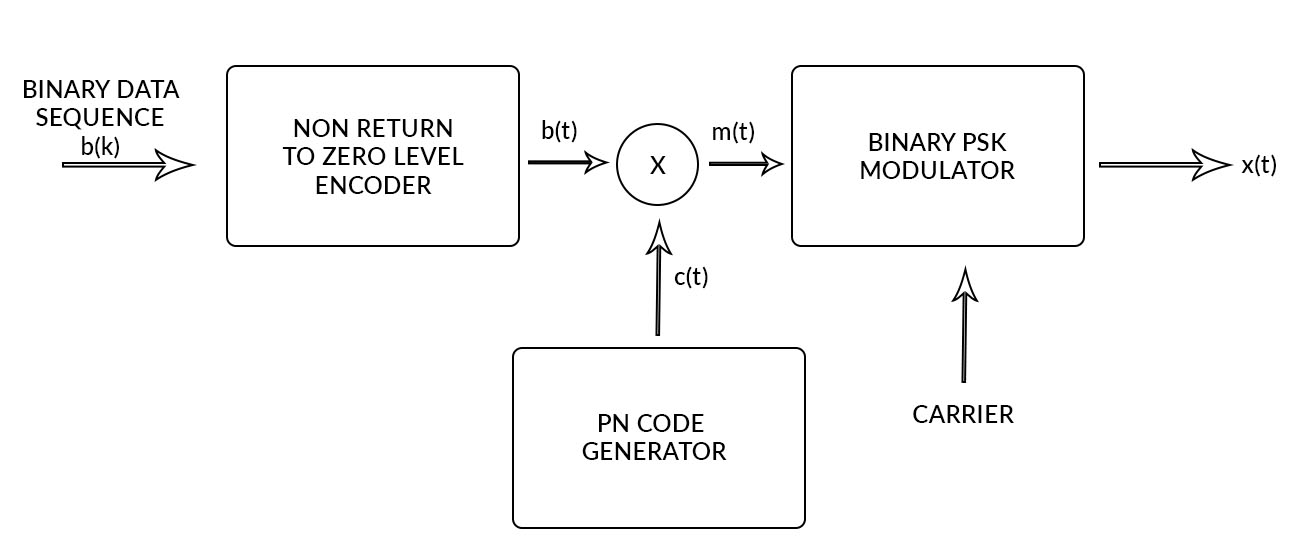
\includegraphics[width=17cm, height=7cm]{Transmitter}\\
\section*{Receiver}
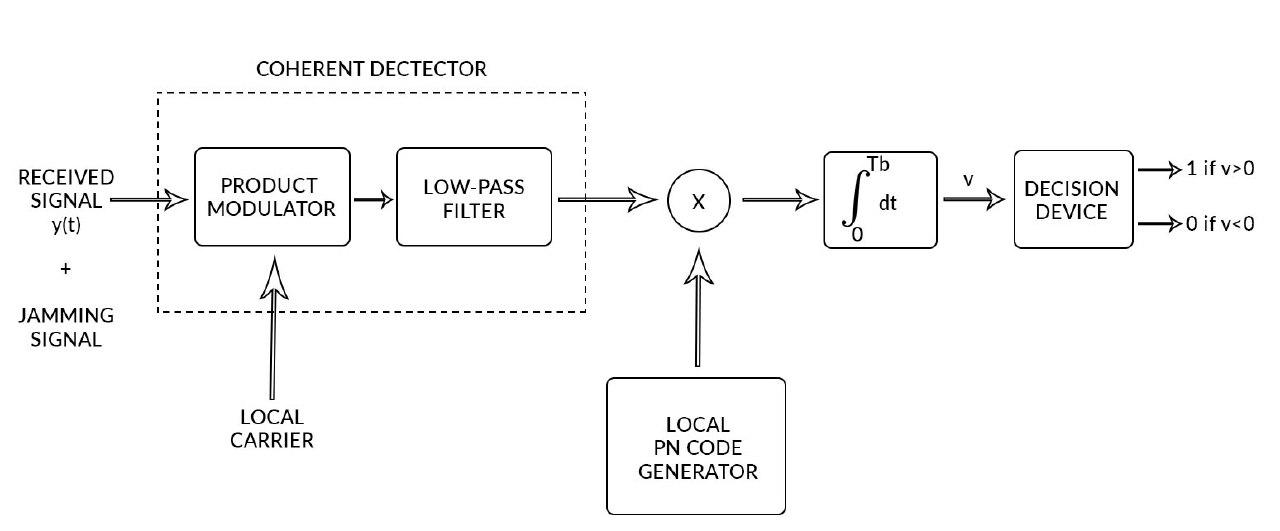
\includegraphics[width=17cm, height=8cm]{Receiver}\\
\end{center}

\begin{flushleft}
\vspace*{1cm}
\section{\fontfamily{qcs}\selectfont EQUATIONS :}
\end{flushleft}

\begin{Large}
\begin{flushleft}
$Non-Zero\ \ level\ \ encoder\ \ : \ \ 2*Binary\ \ input\ \ sequence -1$
$\vspace*{1mm}$
$PN\ \ sequence\ \ : \ \ 1+D6+D7$
$\vspace*{1mm}$\\
$Basis\ \ function\ \ of\ \ carrier = \sqrt\frac{2}{Tb}\cos(2\pi f_ct)$
$\vspace*{1mm}$\\
$Probability\ \ of\ \ error\ \ :\  \frac{1}{2}erfc(\sqrt\frac{Eb}{N0})$
$\vspace*{1mm}$\\
$BPSK signal\ \ : \ x(t)=b(t)\sqrt{Eb}\sqrt\frac{2}{Tb}\cos(2\pi f_ct)$\\
\vspace*{0.1mm}

\begin{equation*}
 \hspace{-4cm}
where \     \ b(t) : Bipolar signal = 
\begin{cases}
  1\  \ \text{for }1\\    
 -1\  \ \text{for }0\\ 
\end{cases}
\end{equation*}

\begin{equation*}
 \hspace{-5cm}
 \sqrt{Eb} :Energy\ \ of\ \ one\ \ bit 
\end{equation*}



\end{flushleft}
\end{Large}


\begin{flushleft}
\vspace*{1cm}
\section{\fontfamily{qcs}\selectfont PYTHON CODE :}
\end{flushleft}

\begin{Large}
\begin{flushleft}
\lstset{language=Python}
\lstset{label={lst:code_direct}}
\lstset{basicstyle=\normalsize}

\lstinputlisting[language=Python]{code.py}
\end{flushleft}
\end{Large}

\begin{flushleft}
\vspace*{1cm}
\section{\fontfamily{qcs}\selectfont OBSERVATIONS :}
\end{flushleft}



\begin{center}
\vspace*{1cm}
\large{\textbf{Input Signal}}\\
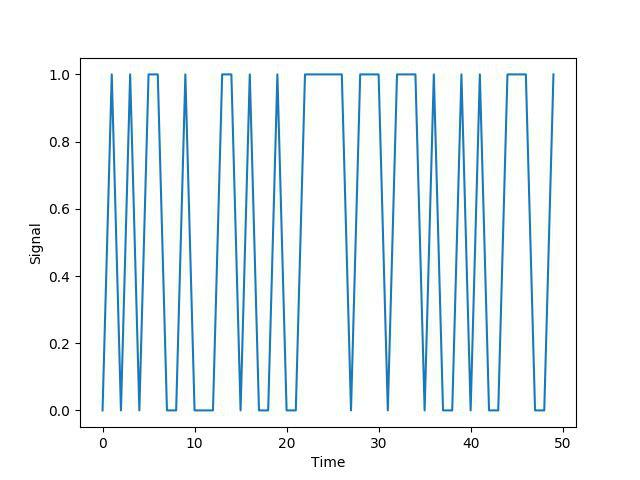
\includegraphics[width=15cm, height=10cm]{fig1}\\

\vspace*{1cm}
\large{\textbf{Carrier Signal}}\\
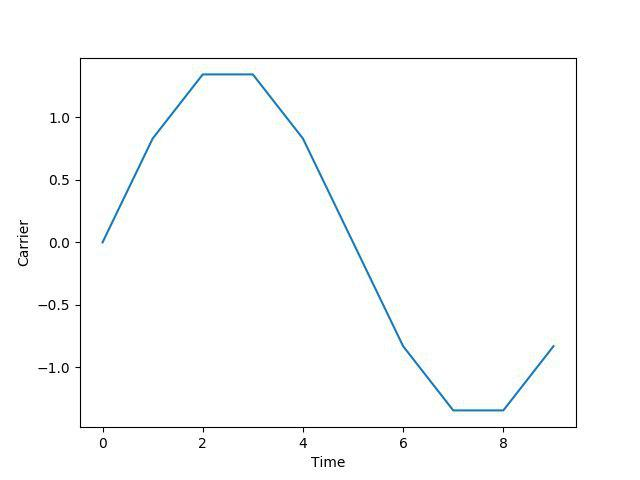
\includegraphics[width=15cm, height=10cm]{fig2}\\
\newpage
\vspace*{1cm}
\large{\textbf{Jamming Signal}}\\
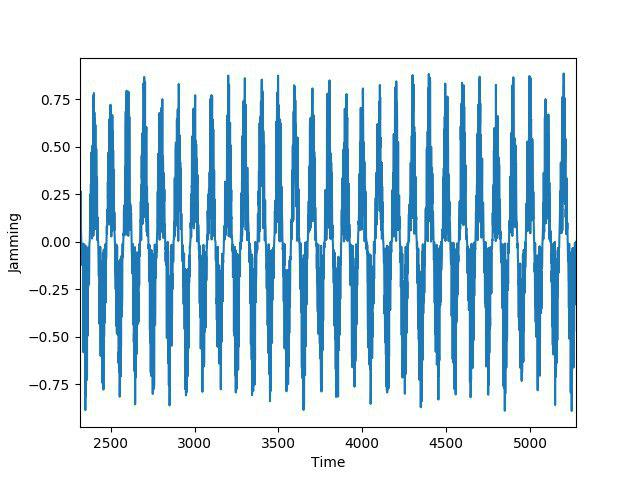
\includegraphics[width=15cm, height=10cm]{fig3}\\
\vspace*{1cm}
\large{\textbf{Bpsk Signal}}\\
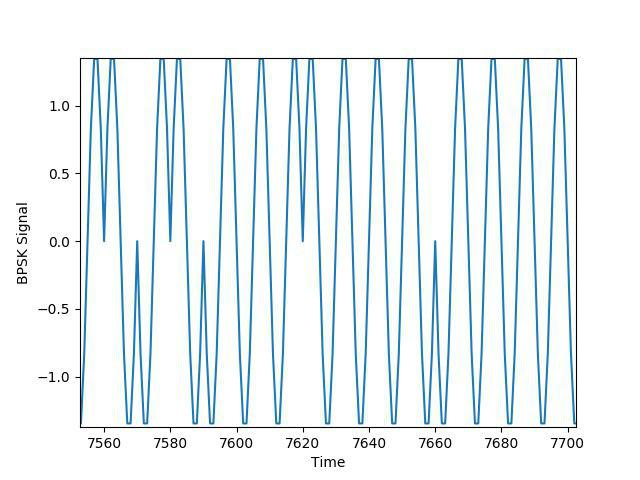
\includegraphics[width=15cm, height=10cm]{fig4}\\
\vspace*{1cm}
\newpage
\large{\textbf{Received Signal}}\\
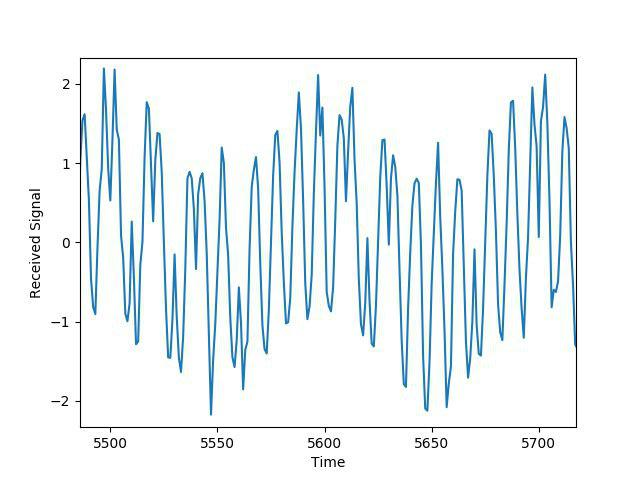
\includegraphics[width=15cm, height=10cm]{fig5}\\
\vspace*{1cm}
\large{\textbf{Bit Error Rate Vs Signal to Noise Ratio}}\\
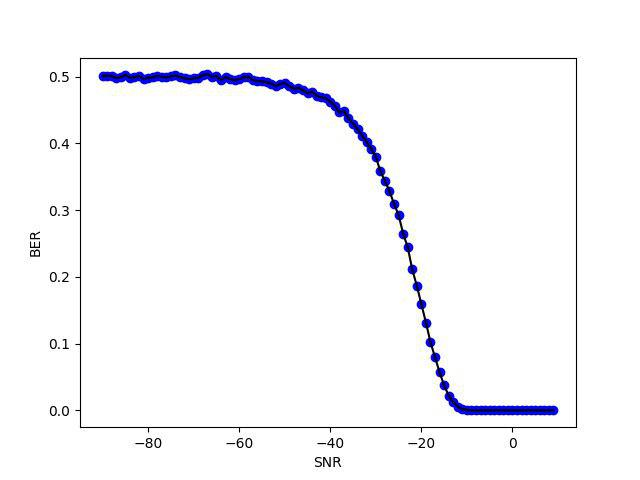
\includegraphics[width=15cm, height=10cm]{fig6}\\
\newpage
\vspace*{1cm}
\large{\textbf{Signal Constellation Without Jamming}}\\
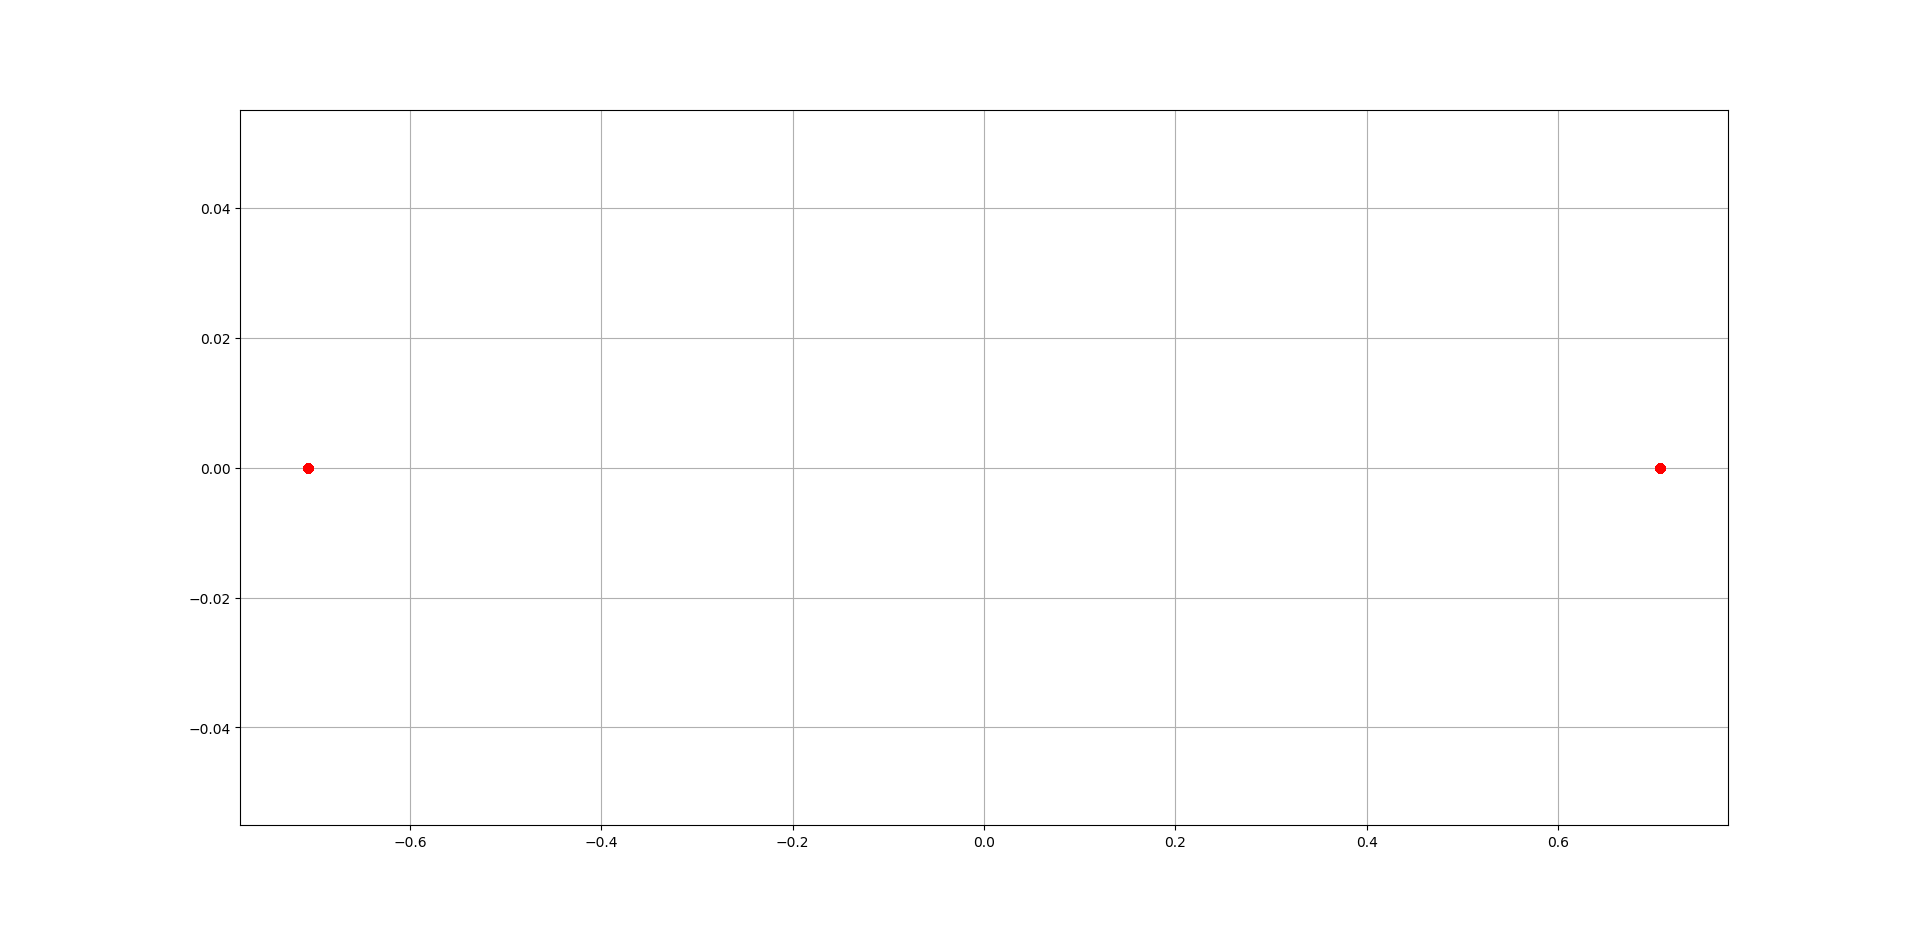
\includegraphics[width=15cm, height=10cm]{fig7}\\
\vspace*{1cm}
\large{\textbf{Signal Constellation With Jamming}}\\
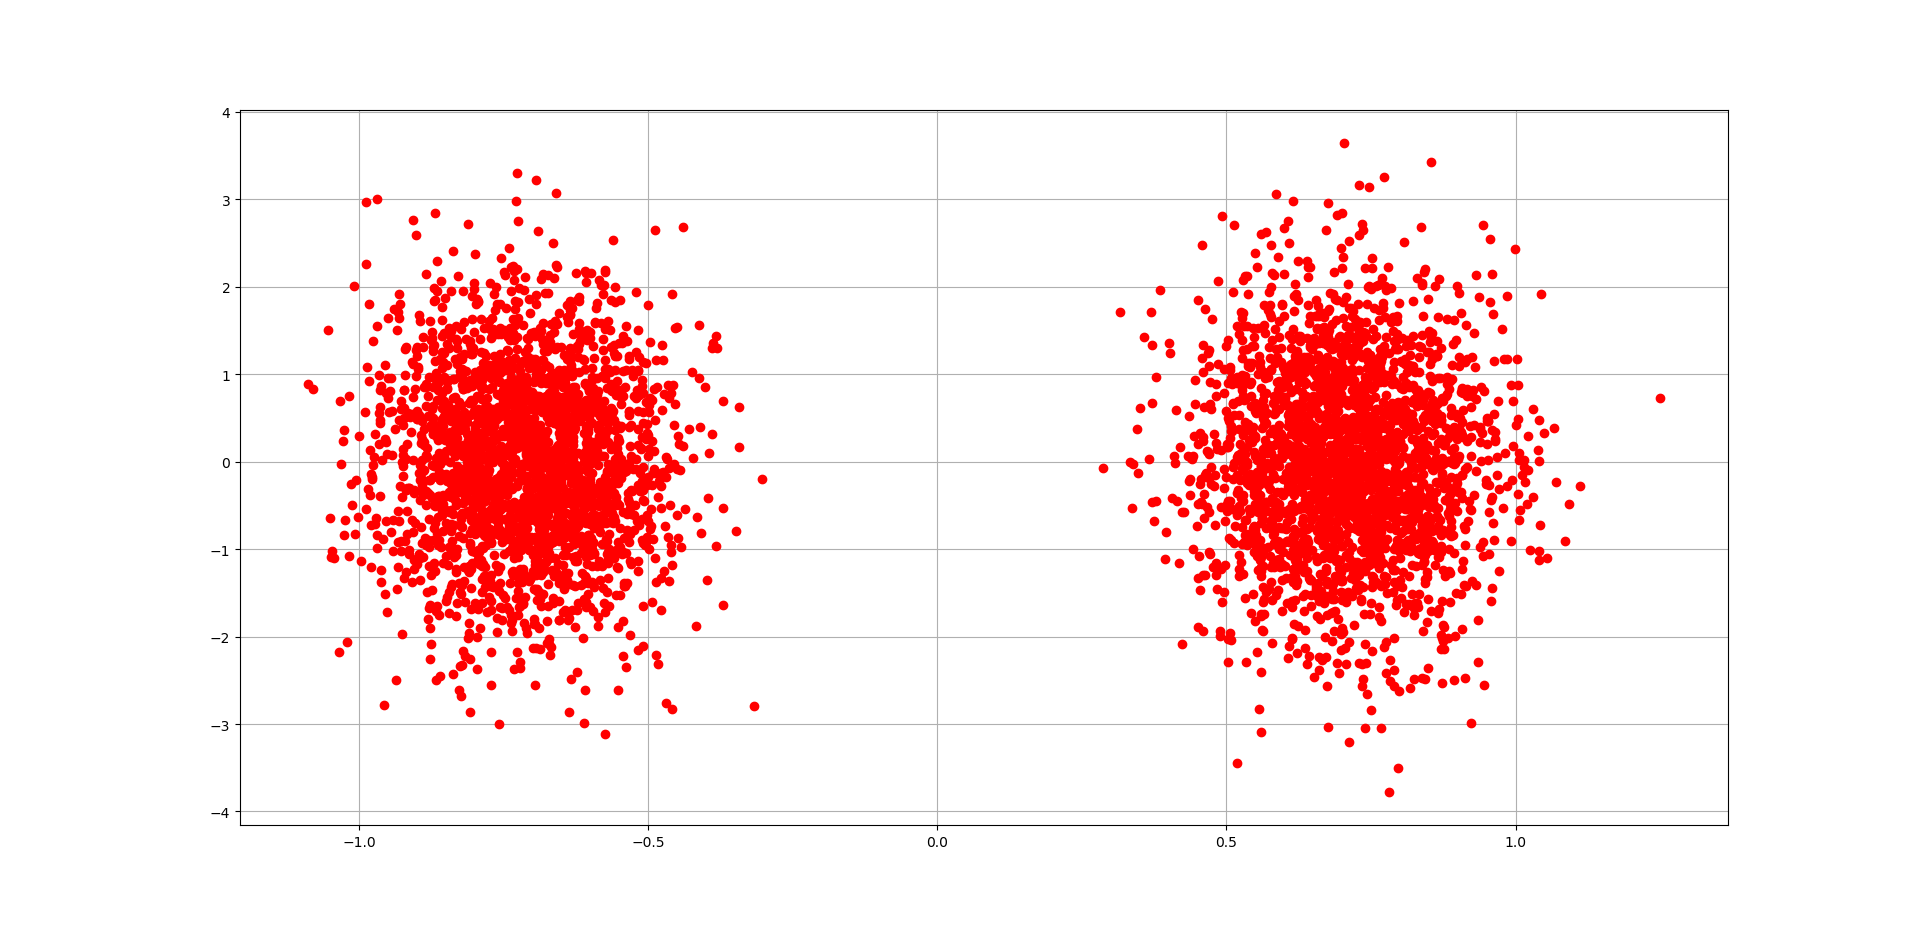
\includegraphics[width=15cm, height=10cm]{fig8}\\

\end{center}

\begin{flushleft}
\vspace*{1cm}
\section{\fontfamily{qcs}\selectfont RESULT :}
\end{flushleft}

\begin{Large}
\begin{center}
Simulated DS-BPSK system in python ( Transmitter and Receiver with PN sequence and Jamming ) and to plot SNR vs BER, Constellation of BPSK.
\end{center}
\end{Large}







  
  
  
  
  
  
  
  
  
  
  
  
  
  
  
  
  
  
  
  
  
  \end{document}
  
